\section{Results and Discussion}
The system underwent a two-minute run, with data sampled every second. During this period, the system was subjected to temperature fluctuations, including pulses, to observe its response. The collected dataset is visualized in Fig~\ref{fig:t_plot}.

\begin{figure}[H]
    \centering
    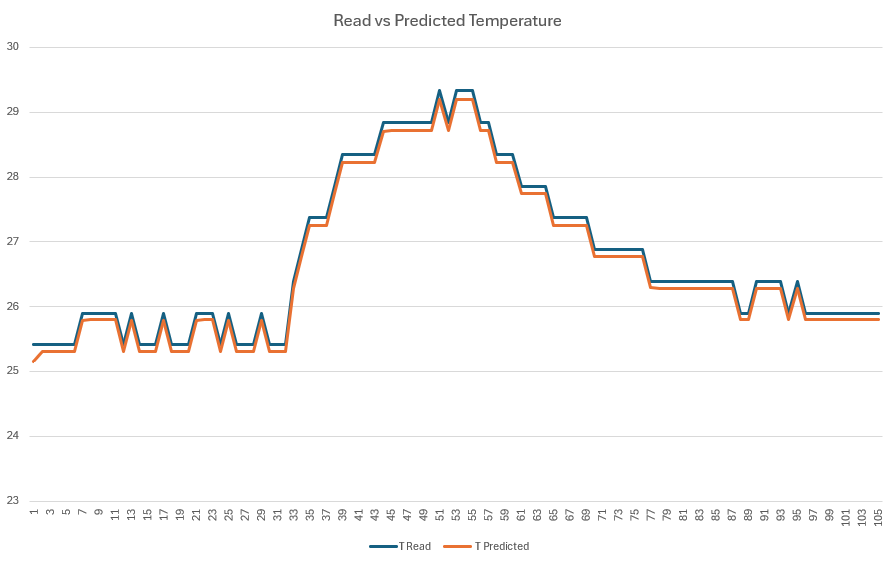
\includegraphics[width=1\linewidth]{figures/t_plot.png}
    \caption{Comparison of the read and the predicted temperature}
~\label{fig:t_plot}
\end{figure}

Using the collected data, the absolute error between the predicted and actual values was calculated, yielding an average error of $0.4\%$, and a maximum error of $1\%$ at the onset of the run. Conversely, the minimum error recorded was $0.3\%$. These results indicate that the system demonstrates robustness and reliability in predicting values, even under dynamic temperature conditions. These findings are summarized in Table~\ref{tab:error_table}.

\begin{table}[H]
\centering
    \begin{tabular}{|c|c|c|c|}
    \hline
    Samples & Average Error & Min Error & Max Error \\ \hline
      105   &     0.4\%     &   0.3\%   &    1\%    \\ \hline
    \end{tabular}
\caption{Summary table for prediction error}
\label{tab:error_table}
\end{table}
